\documentclass[pdflatex,compress]{beamer}

%\usetheme[dark,framenumber,totalframenumber]{ElektroITK}
\usetheme[darktitle,framenumber,totalframenumber]{ElektroITK}

\usepackage[utf8]{inputenc}
\usepackage[T1]{fontenc}
\usepackage{lmodern}
\usepackage[bahasai]{babel}
\usepackage{amsmath}
\usepackage{amsfonts}
\usepackage{amssymb}
\usepackage{graphicx}
\usepackage{multicol}

\title{PEMODELAN JARINGAN KOMUNIKASI}
\subtitle{OSI Layer 2 - The Data Link Layer}

\author{Tim Dosen Pengampu}

\begin{document}

\maketitle

\begin{frame}
	\frametitle{Layer 2 – The Data Link Layer}
	\begin{itemize}
		\item Frames are encoded and decoded into bits at Layer 2.
		\item Error detection and correction for the Physical Layer can be provided here.
		\item Ethernet is the Layer 2 medium used on Local Area Networks.
		\item List of network protocol (OSI Model) \href{https://en.wikipedia.org/wiki/List_of_network_protocols_(OSI_model)}{\beamergotobutton{Link}} 
	\end{itemize}
\end{frame}

\begin{frame}
	\frametitle{OSI Reference Model - Encapsulation}
	\begin{center}
		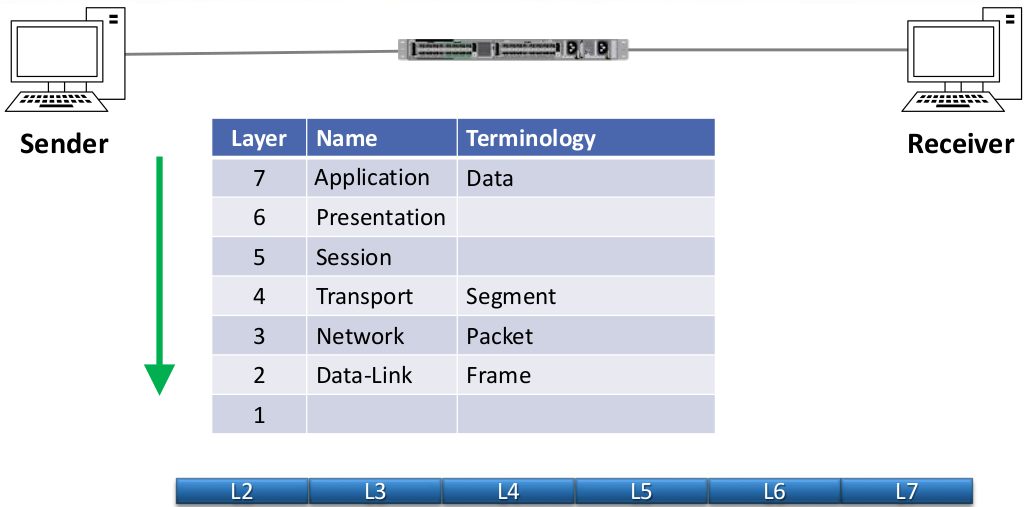
\includegraphics[width=\linewidth]{img/img01}
	\end{center}
\end{frame}

\begin{frame}
	\frametitle{The Ethernet Header}
	\begin{center}
		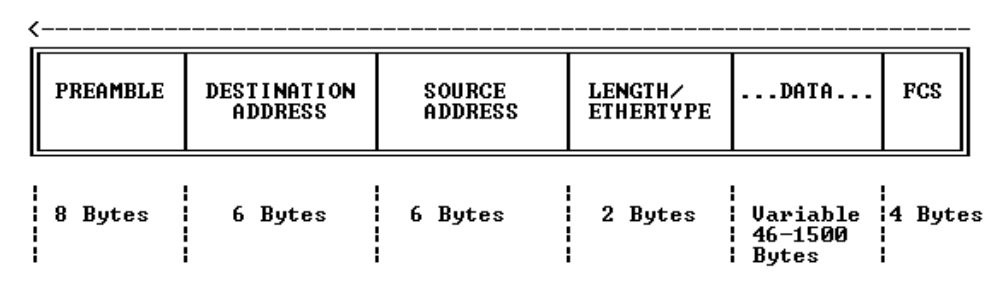
\includegraphics[width=\linewidth]{img/img02}
	\end{center}
	FCS = Frame Check Sequence
\end{frame}

\begin{frame}
	\frametitle{The Media Access Control\\ MAC Address}
	\begin{itemize}
		\item Ethernet uses a 48-bit hexadecimal MAC Address.
		\item The first 24 bits is the OUI (Organizationally Unique Identifier) which uniquely identifies the manufacturer of the Ethernet port. The OUI is assigned by the IEEE.
		\item The last 24 bits is vendor assigned.
		\item The burned in MAC address on every NIC port in the world is globally unique.
		\item Example - 00:50:56:C0:00:08
		\begin{multicols}{2}
			\begin{center}
				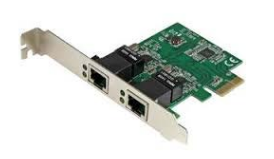
\includegraphics[width=0.8\linewidth]{img/img03}
			\end{center}
			\columnbreak
			The 48-bit address space contains potentially $ 2^48 $ or \textbf{281,474,976,710,656}
			possible MAC addresses.
		\end{multicols}
	\end{itemize}
\end{frame}

\end{document}
